%%%%%%%%%%%%%%%%%%%%%%%%%%%%%%%%%%%%%%%%%%%%%%%%%%%%%%%%%%%%%%%%%%%%%%%%%
%  Zawartość: Główny plik szablonu pracy dyplomowej (magisterskiej/inżynierskiej).
%  Opracował: Tomasz Kubik <tomasz.kubik@pwr.edu.pl>
%  Data: kwiecień 2016
%  Wersja: 0.2
%%%%%%%%%%%%%%%%%%%%%%%%%%%%%%%%%%%%%%%%%%%%%%%%%%%%%%%%%%%%%%%%%%%%%%%%%

\documentclass[a4paper,onecolumn,oneside,12pt,extrafontsizes]{memoir}
% W celu przygotowania wydruku do archiwum należy przesłonić komendę powyższą
% dwoma poniższymi komendami:
%\documentclass[a4paper,onecolumn,twoside,10pt]{memoir} 
%\renewcommand{\normalsize}{\fontsize{8pt}{10pt}\selectfont}
%
%\usepackage[cp1250]{inputenc} % jeśli kodowanie edytowanych plików to cp1250 
%\usepackage[utf8]{inputenc} % jeśli kodowanie edytowanych plików to UTF8
\usepackage[T1]{fontenc}
\usepackage[polish]{babel}
%\DisemulatePackage{setspace}
\usepackage{setspace}
\usepackage{tabularx}
\usepackage{color,calc}
%\usepackage{soul} % pakiet z komendami do podkreślania tekstu

\usepackage{ebgaramond} % pakiet z czcionkami garamond, potrzebny tylko do strony tytułowej, musi wystąpić przed pakietem tgtermes

%% Aby uzyskać polskie literki w pdfie (a nie zlepki) korzystamy z pakietu czcionek tgterms. 
%% W pakiecie tym są zdefiniowane klony czcionek Times o kształtach: normalny, pogrubiony, italic, italic pogrubiony.
%% W pakiecie tym brakuje czcionki o kształcie: slanted (podobny do italic). 
%% Jeśli w dokumencie gdzieś zostanie zastosowana czcionka slanted (np. po użyciu komendy \textsl{}), to
%% latex dokona podstawienia na czcionkę standardową i zgłosi to w ostrzeżeniu (warningu).
%% Ponadto tgtermes to czcionka do tekstu. Wszelkie matematyczne wzory będą sformatowane domyślną czcionką do wzorów.
%% Jeśli wzory mają być sformatowane z wykorzystaniem innych czcionek, trzeba to jawnie zadeklarować.

%% Po zainstalowaniu pakietu tgtermes może będzie trzeba zauktualizować informacje 
%% o dostępnych fontach oraz mapy. Można to zrobić z konsoli (jako administrator)
%% initexmf --admin --update-fndb
%% initexmf --admin --mkmaps

\usepackage{tgtermes}   
\renewcommand*\ttdefault{txtt}

\usepackage{float}

% We wcześniejszej wersji szablonu korzystano z innych czcionek. Dla celów historycznych pozostawiono je w komentarzu
%\usepackage{mathptmx} % pakiet będący następcą pakietów times and mathptm, niestety polskie literki są zlepkami
%\usepackage{newtxtext,newtxmath} % pakiety dostarczające Times dla tekstów i wzorów matematycznych,  
%                                  rozwiązuje problemy występujące w mathptmx, ale wymaga zainstalowania
%                                  dodatkowych pakietów oraz uruchomienia updmap (konsola administratora)
%                                  niestety polskie literki są zlepkami
%\usepackage{newtxmath,tgtermes} % można też połączyć czcionki do tekstu i czcionki do wzorów

\usepackage{listings} % pakiet do prezentacji kodu. 
%Wcześniej był problem z polskimi znakami w otoczeniu lstlisting, stąd pozostawiono w komentarzu zastosowane wtedy rozwiązanie: 
\lstset{literate=%-
{ą}{{\k{a}}}1 {ć}{{\'c}}1 {ę}{{\k{e}}}1 {ł}{{\l{}}}1 {ń}{{\'n}}1 {ó}{{\'o}}1 {ś}{{\'s}}1 {ż}{{\.z}}1 {ź}{{\'z}}1 {Ą}{{\k{A}}}1 {Ć}{{\'C}}1 {Ę}{{\k{E}}}1 {Ł}{{\L{}}}1 {Ń}{{\'N}}1 {Ó}{{\'O}}1 {Ś}{{\'S}}1 {Ż}{{\.Z}}1 {Ź}{{\'Z}}1 }%{\ \ }{{\ }}1}

% Choć możliwe jest zastosowanie różnych pakietów formatujących tabele, zaleca się tego nie robić.
%\usepackage{longtable}
%\usepackage{ltxtable}
%\usepackage{tabulary}

%%%%%%%%%%%%%%%%%%%%%%%%%%%%%%%%%%%%%%%%%%%%%%%%%%%
%% Ustawienia odpowiedzialne za sposób łamania dokumentu
%% i ułożenie elementów pływających
%%%%%%%%%%%%%%%%%%%%%%%%%%%%%%%%%%%%%%%%%%%%%%%%%%%
%\hyphenpenalty=10000		% nie dziel wyrazów zbyt często
\clubpenalty=10000      %kara za sierotki
\widowpenalty=10000  % nie pozostawiaj wdów
\brokenpenalty=10000		% nie dziel wyrazów między stronami
\exhyphenpenalty=999999		% nie dziel słów z myślnikiem
\righthyphenmin=3			% dziel minimum 3 litery

%\tolerance=4500
%\pretolerance=250
%\hfuzz=1.5pt

%\hbadness=1450

\renewcommand{\topfraction}{0.95}
\renewcommand{\bottomfraction}{0.95}
\renewcommand{\textfraction}{0.05}
\renewcommand{\floatpagefraction}{0.35}

%%%%%%%%%%%%%%%%%%%%%%%%%%%%%%%%%%%%%%%%%%%%%%%%%%%
%%  Ustawienia rozmiarów: tekstu, nagłówka i stopki, marginesów
%%  dla dokumentów klasy memoir 
%%%%%%%%%%%%%%%%%%%%%%%%%%%%%%%%%%%%%%%%%%%%%%%%%%%
\setlength{\headsep}{10pt} 
\setlength{\headheight}{13.6pt} % wartość baselineskip dla czcionki 11pt tj. \small wynosi 13.6pt
\setlength{\footskip}{\headsep+\headheight}
\setlength{\uppermargin}{\headheight+\headsep+1cm}
\setlength{\textheight}{\paperheight-\uppermargin-\footskip-1.5cm}
\setlength{\textwidth}{\paperwidth-5cm}
\setlength{\spinemargin}{2.5cm}
\setlength{\foremargin}{2.5cm}
\setlength{\marginparsep}{2mm}
\setlength{\marginparwidth}{2.3mm}
%\settrimmedsize{297mm}{210mm}{*}
%\settrims{0mm}{0mm}	
\checkandfixthelayout[fixed] % konieczne, aby się dobrze wszystko poustawiało
%%%%%%%%%%%%%%%%%%%%%%%%%%%%%%%%%%%%%%%%%%%%%%%%
%%  Ustawienia odległości linii, wcięć, odstępów
%%%%%%%%%%%%%%%%%%%%%%%%%%%%%%%%%%%%%%%%%%%%%%%%
\linespread{1}
%\linespread{1.241}
\setlength{\parindent}{14.5pt}
%\setbeforesecskip{10pt plus 0.5ex}%{-3.5ex \@plus -1ex \@minus -.2ex}
%\setaftersecskip{10pt plus 0.5ex}%\onelineskip}
%\setbeforesubsecskip{8pt plus 0.5ex}%{-3.5ex \@plus -1ex \@minus -.2ex}
%\setaftersubsecskip{8pt plus 0.5ex}%\onelineskip}
%\setlength\floatsep{6pt plus 2pt minus 2pt} 
%\setlength\intextsep{12pt plus 2pt minus 2pt} 
%\setlength\textfloatsep{12pt plus 2pt minus 2pt} 

%%%%%%%%%%%%%%%%%%%%%%%%%%%%%%%%%%%%%%%%%%%%%%%%%%%
%%  Pakiety i komendy zastosowane tylko do zamieszczenia informacji o użytych komendach i fontach
%%  Normalnie nie są potrzebne, można je zamarkować podczas redakcji pracy
%%%%%%%%%%%%%%%%%%%%%%%%%%%%%%%%%%%%%%%%%%%%%%%%%%%
\usepackage{memlays}     % extra layout diagrams, zastosowane w szblonie do 'debuggowania', używa pakietu layouts
%\usepackage{layouts}
\usepackage{printlen} % pakiet do wyświetlania wartości zdefiniowanych długości, stosowany do 'debuggowania'
\uselengthunit{pt}
\makeatletter
\newcommand{\showFontSize}{\f@size pt} % makro wypisujące wielkość bieżącej czcionki
\makeatother
% do pokazania ramek można byłoby użyć:
%\usepackage{showframe} 


%%%%%%%%%%%%%%%%%%%%%%%%%%%%%%%%%%%%%%%%%%%%%%%%%%%
%%  Formatowanie list wyliczeniowych, wypunktowań i własnych otoczeń
%%%%%%%%%%%%%%%%%%%%%%%%%%%%%%%%%%%%%%%%%%%%%%%%%%%

% Domyślnie wypunktowania mają zadeklatorowane znaki, które nie występują w tgtermes
% Aby latex nie podstawiał w ich miejsca znaków z czcionki standardowej można zrobić podstawienie:
%    \DeclareTextCommandDefault{\textbullet}{\ensuremath{\bullet}}
%    \DeclareTextCommandDefault{\textasteriskcentered}{\ensuremath{\ast}}
%    \DeclareTextCommandDefault{\textperiodcentered}{\ensuremath{\cdot}}
% Jednak jeszcze lepszym pomysłem jest zdefiniowanie otoczeń z wykorzystaniem enumitem
\usepackage{enumitem} % pakiet pozwalający zarządzać formatowaniem list wyliczeniowych
\setlist{noitemsep,topsep=4pt,parsep=0pt,partopsep=4pt,leftmargin=*} % zadeklarowane parametry pozwalają uzyskać 'zwartą' postać wypunktowania bądź wyliczenia
\setenumerate{labelindent=0pt,itemindent=0pt,leftmargin=!,label=\arabic*.} % można zmienić \arabic na \alph, jeśli wyliczenia mają być z literkami
\setlistdepth{4} % definiujemy głębokość zagnieżdżenia list wyliczeniowych do 4 poziomów
\setlist[itemize,1]{label=$\bullet$}  % definiujemy, jaki symbol ma być użyty w wyliczeniu na danym poziomie
\setlist[itemize,2]{label=\normalfont\bfseries\textendash}
\setlist[itemize,3]{label=$\ast$}
\setlist[itemize,4]{label=$\cdot$}
\renewlist{itemize}{itemize}{4}

%%%http://tex.stackexchange.com/questions/29322/how-to-make-enumerate-items-align-at-left-margin
%\renewenvironment{enumerate}
%{
%\begin{list}{\arabic{enumi}.}
%{
%\usecounter{enumi}
%%\setlength{\itemindent}{0pt}
%%\setlength{\leftmargin}{1.8em}%{2zw} % 
%%\setlength{\rightmargin}{0zw} %
%%\setlength{\labelsep}{1zw} %
%%\setlength{\labelwidth}{3zw} % 
%\setlength{\topsep}{6pt}%
%\setlength{\partopsep}{0pt}%
%\setlength{\parskip}{0pt}%
%\setlength{\parsep}{0em} % 
%\setlength{\itemsep}{0em} % 
%%\setlength{\listparindent}{1zw} % 
%}
%}{
%\end{list}
%}

\makeatletter
\renewenvironment{quote}{
	\begin{list}{}
	{
	\setlength{\leftmargin}{1em}
	\setlength{\topsep}{0pt}%
	\setlength{\partopsep}{0pt}%
	\setlength{\parskip}{0pt}%
	\setlength{\parsep}{0pt}%
	\setlength{\itemsep}{0pt}
	}
	}{
	\end{list}}
\makeatother

%%%%%%%%%%%%%%%%%%%%%%%%%%%%%%%%%%%%%%%%%
%%  Pakiet do generowania indeksu (ważne, aby wstawić przed hyperref)
%%%%%%%%%%%%%%%%%%%%%%%%%%%%%%%%%%%%%%%%%
\DisemulatePackage{imakeidx}
\usepackage[makeindex,noautomatic]{imakeidx} % tutaj mówimy, żeby indeks nie generował się automatycznie, 

%\usepackage[noautomatic]{imakeidx} 
\makeindex

\makeatletter
%%%\renewenvironment{theindex}
							 %%%{\vskip 10pt\@makeschapterhead{\indexname}\vskip -3pt%
								%%%\@mkboth{\MakeUppercase\indexname}%
												%%%{\MakeUppercase\indexname}%
								%%%\vspace{-3.2mm}\parindent\z@%
								%%%\renewcommand\subitem{\par\hangindent 16\p@ \hspace*{0\p@}}%%
								%%%\phantomsection%
								%%%\begin{multicols}{2}
								%%%%\thispagestyle{plain}
								%%%\parindent\z@                
								%%%%\parskip\z@ \@plus .3\p@\relax
								%%%\let\item\@idxitem}
							 %%%{\end{multicols}\clearpage}
%%%
\makeatother


\usepackage{ifpdf}
%\newif\ifpdf \ifx\pdfoutput\undefined
%\pdffalse % we are not running PDFLaTeX
%\else
%\pdfoutput=1 % we are running PDFLaTeX
%\pdftrue \fi
\ifpdf
 \usepackage[pdftex,bookmarks,breaklinks,unicode]{hyperref}
 \usepackage[pdftex]{graphicx}
 \DeclareGraphicsExtensions{.pdf,.jpg,.mps,.png}
\pdfcompresslevel=9
\pdfoutput=1
\makeatletter
\AtBeginDocument{
  \hypersetup{
	pdfinfo={
    Title = {\@title},
    Author = {\@author},
    Subject={},
    Keywords={słowa kluczowe},
  }}
}
\makeatother
\else
\usepackage{graphicx}
\DeclareGraphicsExtensions{.eps,.ps,.jpg,.mps,.png}
\fi
\sloppy


%\graphicspath{{rys01/}{rys02/}}


%%%%%%%%%%%%%%%%%%%%%%%%%%%%%%%%%%%%%%%%%
% Metadane dla pdfa


%\ifpdf
%\pdfinfo{
   %/Author (Nicola Talbot)
   %/Title  (Creating a PDF document using PDFLaTeX)
   %/CreationDate (D:20040502195600)
   %/ModDate (D:\pdfdate)
   %/Subject (PDFLaTeX)
   %/Keywords (PDF;LaTeX)
%}
%\fi

% Deklaracja głębokościu numeracji
\setcounter{secnumdepth}{2}
\setcounter{tocdepth}{2}
\setsecnumdepth{subsection} % activating subsubsec numbering in doc


% Kropki po numerach sekcji
\makeatletter
\def\@seccntformat#1{\csname the#1\endcsname.\quad}
\def\numberline#1{\hb@xt@\@tempdima{#1\if&#1&\else.\fi\hfil}}
\makeatother

\renewcommand{\chapternumberline}[1]{#1.\quad}
\renewcommand{\cftchapterdotsep}{\cftdotsep}

%\definecolor{niceblue}{rgb}{.168,.234,.671}

% Czcionka do podpisów tabel i rysunków
\captionnamefont{\small}
\captiontitlefont{\small}
% makro pozwalające zmienić sposób wypisywania rozdziału
%\def\printchaptertitle##1{\fonttitle \space \thechapter.\space ##1} 

%\usepackage{ltcaption}
% The ltcaption package supports \CaptionLabelFont & \CaptionTextFont introduced by the NTG document classes
%\renewcommand\CaptionLabelFont{\small}
%\renewcommand\CaptionTextFont{\small}

% Przedefiniowanie etykiet w podpisach tabel i rysunków
%\AtBeginDocument{% 
        \addto\captionspolish{% 
        \renewcommand{\tablename}{Tab.}% 
}%} 

%\AtBeginDocument{% 
%        \addto\captionspolish{% 
%        \renewcommand{\chaptername}{Rozdział}% 
%}} 

%\AtBeginDocument{% 
        \addto\captionspolish{% 
        \renewcommand{\figurename}{Rys.}% 
}%}


%\AtBeginDocument{% 
        \addto\captionspolish{% 
        \renewcommand{\bibname}{Literatura}% 
}%}

%\AtBeginDocument{% 
        \addto\captionspolish{% 
        \renewcommand{\listfigurename}{Spis rysunków}% 
}%}

%\AtBeginDocument{% 
        \addto\captionspolish{% 
        \renewcommand{\listtablename}{Spis tabel}% 
}%}

%\AtBeginDocument{% 
        \addto\captionspolish

%%%%%%%%%%%%%%%%%%%%%%%%%%%%%%%%%%%%%%%%%%%%%%%%%%%%%%%%%%%%%%%%%%                  
%% Definicje stopek i nagłówków
%%%%%%%%%%%%%%%%%%%%%%%%%%%%%%%%%%%%%%%%%%%%%%%%%%%%%%%%%%%%%%%%%%                  
\addtopsmarks{headings}{%
\nouppercaseheads % added at the beginning
}{%
\createmark{chapter}{both}{shownumber}{}{. \space}
%\createmark{chapter}{left}{shownumber}{}{. \space}
\createmark{section}{right}{shownumber}{}{. \space}
}%use the new settings

\makeatletter
\copypagestyle{outer}{headings}
\makeoddhead{outer}{}{}{\small\itshape\rightmark}
\makeevenhead{outer}{\small\itshape\leftmark}{}{}
\makeoddfoot{outer}{\small\@author:~\@titleShort}{}{\small\thepage}
\makeevenfoot{outer}{\small\thepage}{}{\small\@author:~\@title}
\makeheadrule{outer}{\linewidth}{\normalrulethickness}
\makefootrule{outer}{\linewidth}{\normalrulethickness}{2pt}
\makeatother

% fix plain
\copypagestyle{plain}{headings} % overwrite plain with outer
\makeoddhead{plain}{}{}{} % remove right header
\makeevenhead{plain}{}{}{} % remove left header
\makeevenfoot{plain}{}{}{}
\makeoddfoot{plain}{}{}{}

\copypagestyle{empty}{headings} % overwrite plain with outer
\makeoddhead{empty}{}{}{} % remove right header
\makeevenhead{empty}{}{}{} % remove left header
\makeevenfoot{empty}{}{}{}
\makeoddfoot{empty}{}{}{}


%%%%%%%%%%%%%%%%%%%%%%%%%%%%%%%%%%%%%%%
%% Definicja strony tytułowej 
%%%%%%%%%%%%%%%%%%%%%%%%%%%%%%%%%%%%%%%
\makeatletter
%Uczelnia
\newcommand\uczelnia[1]{\renewcommand\@uczelnia{#1}}
\newcommand\@uczelnia{}
%Wydział
\newcommand\wydzial[1]{\renewcommand\@wydzial{#1}}
\newcommand\@wydzial{}
%Kierunek
\newcommand\kierunek[1]{\renewcommand\@kierunek{#1}}
\newcommand\@kierunek{}
%Specjalność
\newcommand\specjalnosc[1]{\renewcommand\@specjalnosc{#1}}
\newcommand\@specjalnosc{}
%Tytuł po angielsku
\newcommand\titleEN[1]{\renewcommand\@titleEN{#1}}
\newcommand\@titleEN{}
%Tytuł krótki
\newcommand\titleShort[1]{\renewcommand\@titleShort{#1}}
\newcommand\@titleShort{}
%Promotor
\newcommand\promotor[1]{\renewcommand\@promotor{#1}}
\newcommand\@promotor{}

%\usepackage[absolute]{textpos} % zamarkowano, bo ostatecznie wykorzystano otoczenie picture

\def\maketitle{%
  \pagestyle{empty}%
%%\garamond 
	\fontfamily{\ebgaramond@family}\selectfont % na stronie tytułowej czcionka garamond
%%%%%%%%%%%%%%%%%%%%%%%%%%%%%%%%%%%%%	
%% Poniżej, w otoczniu picture, wstawiono tytuł i autora. 
%% Tytuł (z autorem) musi znaleźć się w obszarze 
%% odpowiadającym okienku 110mmx75mm, którego lewy górny róg 
%% jest w położeniu 77mm od lewej i 111mm od górnej  krawędzi strony 
%% (tak wynika z wycięcia na okładce). 
%% Poniższy kod musi być użyty dokładnie w miejscu gdzie jest.
%% Jeśli tytuł nie mieści się w okienku, to należy tak pozmieniać 
%% parametry użytych komend, aby ten przydługi tytuł jednak 
%% upakować go do okienka.
%%
%% Sama okładka (kolorowa strona z wycięciem, do pobrania z dydaktyki) 
%% powinna być przycięta o 3mm od każdej z krawędzi.
%% Te 3mm pewnie zostawiono na ewentualne spady czy też specjalną oprawę.
%%%%%%%%%%%%%%%%%%%%%%%%%%%%%%%%%%%%%	
\newlength{\tmpfboxrule}
\setlength{\tmpfboxrule}{\fboxrule}
\setlength{\fboxsep}{2mm}
\setlength{\fboxrule}{0mm} 
%\setlength{\fboxrule}{0.1mm} %% jeśli chcemy zobaczyć ramkę
\setlength{\unitlength}{1mm}
\begin{picture}(0,0)
\put(26,-124){\fbox{
\parbox[c][71mm][c]{104mm}{\centering%\lineskip=34pt 
\fontsize{16pt}{18pt}\selectfont \@title\\[5mm]
\fontsize{16pt}{18pt}\selectfont \@titleEN\\[20mm]
\fontsize{16pt}{18pt}\selectfont AUTOR:\\[2mm]
\fontsize{14pt}{16pt}\selectfont \@author}
}
}
\end{picture}
\setlength{\fboxrule}{\tmpfboxrule} 
%%%%%%%%%%%%%%%%%%%%%%%%%%%%%%%%%%%%%
%% Reszta strony z nazwą uczelni, wydziału, kierunkiem, specjalnością
%% promotorem, oceną pracy, miastem i rokiem
	{\centering%\vspace{-1cm}
		{\fontsize{22pt}{24pt}\selectfont \@uczelnia}\\[0.4cm]
		{\fontsize{22pt}{24pt}\selectfont \@wydzial}\\[0.5cm]
		  \hrule %\vspace*{0.7cm}
	}
{\flushleft\fontsize{14pt}{16pt}\selectfont%
\begin{tabular}{ll}
KIERUNEK: & \@kierunek\\
SPECJALNOŚĆ: & \@specjalnosc\\
\end{tabular}\\[1.3cm]
}
{\centering
{\fontsize{32pt}{36pt}\selectfont PRACA DYPLOMOWA}\\[0.5cm]
{\fontsize{32pt}{36pt}\selectfont INŻYNIERSKA}\\[2.5cm]
}
\vfill
\begin{tabularx}{\linewidth}{p{6cm}l}
		&{\fontsize{16pt}{18pt}\selectfont PROWADZĄCY PRACĘ:}\\[2mm] %UWAGA: tutaj jest miejsce na nazwisko promotora pracy
		&{\fontsize{14pt}{16pt}\selectfont \@promotor}\\[10mm]
		&{\fontsize{16pt}{18pt}\selectfont OCENA PRACY:}\\[20mm]
	\end{tabularx}
\vspace{2cm}
\hrule\vspace*{0.3cm}
{\centering
{\fontsize{16pt}{18pt}\selectfont \@date}\\[0cm]
}
%\ungaramond
\normalfont
 \cleardoublepage
}
\makeatother
%%%%%%%%%%%%%%%%%%%%%%%%%%%%%%%%%%%%%%%%%

%\AtBeginDocument{\addtocontents{toc}{\protect\thispagestyle{empty}}}


%%%%%%%%%%%%%%%%%%%%%%%%%%%%%%%%%%%%%%%%%
%%  Metadane dokumentu 
%%%%%%%%%%%%%%%%%%%%%%%%%%%%%%%%%%%%%%%%%
\title{Platforma internetowa zrzeszająca zawodników uprawiających amatorsko sporty zespołowe}
\titleShort{Platforma internetowa zrzeszająca zawodników uprawiających amatorsko sporty...}
\titleEN{Web platform for players practicing amateur team sports}
\author{Bartosz Pogoda}
\uczelnia{POLITECHNIKA WROCŁAWSKA}
\wydzial{WYDZIAŁ ELEKTRONIKI}
\kierunek{INFORMATYKA}
\specjalnosc{INŻYNIERIA SYSTEMÓW INFORMATYCZNYCH}
\promotor{dr inż. Marek Piasecki, Jednostka????}
\date{WROCŁAW, 2018}

% Ustawienie odstępu od góry w nienumerowanych rozdziałach oraz wykazach:
% Spis treści, Spis tabel, Spis rysunków, Indeks rzeczowy

%\newlength{\linespace}
%\setlength{\linespace}{-\beforechapskip-\topskip+\headheight+\topsep}
%\makechapterstyle{noNumbered}{%
%\renewcommand\chapterheadstart{\vspace*{\linespace}}
%}

%% powyższa komenda załatwia to, co robią komendy poniższe dla spisów
%\renewcommand*{\tocheadstart}{\vspace*{\linespace}}
%\renewcommand*{\lotheadstart}{\vspace*{\linespace}}
%\renewcommand*{\lofheadstart}{\vspace*{\linespace}}

%%%%%%%%%%%%%%%%%%%%%%%%%%%%%%%%%%%%%%%%%
%                  Początek dokumentu 
%%%%%%%%%%%%%%%%%%%%%%%%%%%%%%%%%%%%%%%%%
%\includeonly{skroty,rozdzial01} % jeśli chcemy kompilować tylko fragmenty, to można tu je wpisać

\begin{document}
% Tutaj można przełączyć odstęp między liniami
%\SingleSpacing
%\OnehalfSpacing
%\DoubleSpacing

%\settypeoutlayoutunit{cm} % do debugowania
%\typeoutstandardlayout    % wypisuje na stdout informacje o ustawieniach
\maketitle

\newpage
\thispagestyle{empty}
\mbox{}\vfill
\noindent\begin{tabular}{@{}ll} Opracował: & Tomasz Kubik <tomasz.kubik@pwr.edu.pl>\\
 Data: & maj 2016 
 \end{tabular}\\[15mm]
\noindent
\includegraphics[width=3cm]{by-nc-sa}\newline
{\normalfont 
Szablon jest udostępniany na licencji Creative Commons: \emph{Uznanie autorstwa -- Użycie niekomercyjne -- Na tych samych warunkach, 3.0 Polska}, Wrocław 2016. \\[2pt]
Oznacza to, że wszystkie zawarte  nim treści można kopiować i  wykorzystywać do celów niekomercyjnych, a także tworzyć na ich podstawie utwory zależne pod warunkiem podania autora i~nazwy licencjodawcy oraz udzielania na utwory zależne takiej samej licencji. Tekst licencji jest dostępny pod adresem: \url{http://creativecommons.org/licenses/by-nc-sa/3.0/pl/}.}
\newpage


\chapterstyle{noNumbered}
\pagestyle{outer}
\mbox{}\pdfbookmark[0]{Spis treści}{spisTresci.1}
\tableofcontents* 

\newpage
\mbox{}\pdfbookmark[0]{Spis rysunków}{spisRysunkow.1}
%\addcontentsline{toc}{chapter}{Spis rysunków}
\listoffigures*
\begin{flushleft}

\end{flushleft}
%{%
%\let\oldnumberline\numberline%
%\renewcommand{\numberline}{\figurename~\oldnumberline}%
%\listoffigures%
%}


\newpage
\mbox{}\pdfbookmark[0]{Spis tabel}{spisTabel.1}
%\addcontentsline{toc}{chapter}{Spis tabel}
\listoftables*

%\chapter*{Skróty}\mbox{}\pdfbookmark[0]{Skróty}{skroty.1}
\label{sec:skroty}
\noindent
\begin{description}
  \item [OGC] (ang.\ \emph{Open Geospatial Consortium}) %-- jednostka arytmetyczno--logiczna
  \item [XML] (ang.\ \emph{eXtensible Markup Language})
  \item [SOAP] (ang.\ \emph{Simple Object Access Protocol})
  \item [WSDL] (ang.\ \emph{Web Services Description Language})
  \item [UDDI] (ang.\ \emph{Universal Description Discovery and Integration})
  \item [GIS] (ang.\ \emph{Geographical Information System})
  \item [SDI] (ang.\ \emph{Spatial Data Infrastructure})
  \item [ISO] (ang.\ \emph{International Standards Organization})
  \item [WMS] (ang.\ \emph{Web Map Service})
  \item [WFS] (ang.\ \emph{Web Feature Service})
  \item [WPS] (ang.\ \emph{Web Processing Service})
  \item [GML] (ang.\ \emph{Geography Markup Language})
  \item [SRG] (ang.\ \emph{Seeded Region Growing})
  \item [SOA] (ang.\ \emph{Service Oriented Architecture })
  \item [IT] (ang.\ \emph{Information Technology })
\end{description}
 %skróty można sobie pominąć
\chapterstyle{default}
\chapter{Wstęp}
\section{Wprowadzenie}

Sport jest aspektem towarzyszącym ludzkości od najdawniejszych czasów. Sprawność fizyczna była niezwykle ważną cechą już dla ludzi pierwotnych, dla których niejednokrotnie mogła ona być czynnikiem decydującym o przetrwaniu. W dalszych dziejach ludzkości duży wpływ na narodziny oraz rozwój kultury fizycznej miały starożytne państwa, które organizowały Igrzyska Sportowe.

Ewolucja sportu trwa nadal. Badania wykazują duży wpływ aktywnego trybu życia na zdrowie fizyczne oraz psychiczne człowieka. Aktywność fizyczna jest nieustannie promowana przez lekarzy oraz inne instytucje. Ogromny wpływ na popularyzację zdrowego trybu życia mają również wszelkie organizowane zawody sportowe, które są bardzo popularne w mediach.

Szczególną dziedziną sportu są sporty zespołowe, w których po za indywidualnymi zdolnościami zawodników, ogromne znaczenie ma współpraca. Umiejętność współdziałania w celu osiągnięcia wspólnego celu jest niezwykle istotną cechą, przydatną w wielu życiowych sytuacjach. Wiele sportów zespołowych swój fenomen opiera również na rywalizacji, która daje zawodnikom dodatkową motywację do samorozwoju.

Sporty zespołowe są od wielu lat promowane poprzez organizację dużych imprez takich jak Mistrzostwa Świata, Mistrzostwa Europy. Wraz z popularnością sportów zespołowych rośnie liczba osób, które uprawiają sporty zespołowe amatorsko\footnote{Amatorsko czyli traktując sport jako hobby, dodatek do życia, a nie jego główny kierunek i źródło utrzymania}. Osoby takie poprzez wspólną grę oraz rywalizację mogą poprawić swoją sprawność fizyczną aktywnie spędzając czas, jak również nawiązać nowe znajomości.

Popularyzacja aktywnego trybu życia w społeczeństwie stanowi motywację oraz uzasadnienie zapotrzebowania na rozwiązania, które przy użyciu technologii dostępnych w dzisiejszych czasach, wspierałyby komunikację pomiędzy osobami uprawiającymi amatorsko sporty zespołowe. 

W celu zapewnienia dużej dostępności rozwiązania bez względu na sprzęt oraz położenie użytkownika naturalnym wyborem jest umieszczenie platformy w Internecie, do którego dostęp ma znaczna większość populacji. Istniejące platformy internetowe takie jak Facebook, YouTube sukcesywnie wspomagają budowanie społeczności ludzi o wspólnych zainteresowaniach, w dużej mierze ze względu na swoją szeroką dostępność.

\section{Cel i zakres pracy}

Celem niniejszej pracy jest zaprojektowanie oraz implementacja prototypu platformy internetowej, która zrzeszałaby osoby uprawiające sporty zespołowe w sposób amatorski poprzez:

\begin{itemize}
  \item utrzymywanie bazy zawodników,
  \item utrzymywanie bazy drużyn,
  \item utrzymywanie bazy obiektów sportowych,
  \item wspomaganie poszukiwania rywali,
  \item wspomaganie umawiania się na rozgrywkę.
\end{itemize} 

Do zakresu pracy należy projekt ogólnego rozwiązania, które mogłoby z powodzeniem być zastosowane dla różnych dyscyplin sportów zespołowych. Implementacja zostanie jednak zrealizowana dla wybranej dyscypliny.

\begin{comment}
Ze względu na duży rozwój

TODO O tym że projekt ogólny a implementacja dla wybranej dziedziny a konkretnie koszykówki 3 na 3 która budzi co raz większe zainteresowanie i np będzie na igrzyskach olimpijskich. Wybór ze względu na popularność dyscypliny i brak dla niej istniejącego rozwiązania\cite{JS07}).
\end{comment}


\section{Układ pracy}

W kolejnym rozdziale niniejszej pracy przedstawiono wybrane z istniejących platform (?). W trzecim rozdziale zawarto koncept rozwiązania. Czwarty rozdział obejmuje projekt systemu. Piąty rozdział przybliża architekturę systemu oraz technologie wybrane do jego budowy. W następnym, szóstym, rozdziale

O układzie pracy, przejście od przeglądu rozwiązań poprzez koncept, projekt techniczny aż do szczegółów implementacji oraz jej walidacji środowiskowej.

\begin{enumerate}
\item xd
\end{enumerate}
\chapter{Istniejące rozwiązania}

W niniejszym rozdziale przedstawione zostały wybrane z istniejących rozwiązań wspierających komunikację pomiędzy zawodnikami. Dla poszczególnych platform zostaną wyszczególnione ich główne założenia oraz sposób w jaki realizują cele podobne systemu będącego przedmiotem tej pracy.


\section{Facebook}

Facebook jest serwisem społecznościowym zrzeszającym prawie 2 miliardy osób z całego świata. Główną misją Facebooka jest zbliżanie do siebie ludzi poprzez umożliwianie budowy społeczności \cite{fb}.

Społeczność osób uprawiających sporty zespołowe nie stanowi tutaj wyjątku. Na Facebooku istnieje bardzo dużo grup tematycznych, których celem jest gromadzenie osób uprawiających pewną dyscyplinę sportu w określonym regionie. Osoby szukające osób do gry bardzo często tworzą posty podając takie informacje jak miejsce oraz termin spotkania, preferowany wiek oraz poziom umiejętności. Chętne osoby zgłaszają się pod postem lub poprzez wiadomość prywatną. Przykładowy post został przedstawiony na rysunku \ref{fig:ss-fb}.

Szukanie osób do gry poprzez portal Facebook jest bardzo często wybieranym rozwiązaniem głownie ze względu na dużą ilość użytkowników oraz szeroką dostępność serwisu. W tabeli \ref{tab:fbgrupy} przedstawiono zestawienie wybranych z publicznych grup w mieście Wrocław


\begin{table}[htb]
\centering\small
\caption{Przykładowe grupy dla zawodników na Facebook - stan z dnia 20.11.2018r}
\label{tab:fbgrupy}
\begin{tabularx}{\linewidth}{|p{.55\linewidth}|X|}\hline
Nazwa grupy & Liczba członków \\ \hline\hline
Piłka nożna Wrocław & 4689  \\ \hline
Siatkówka Wrocław & 4460  \\ \hline
Koszykówka Wrocław & 1686 \\ \hline
Piłka nożna Wrocław - dla PWR & 273  \\ \hline
\end{tabularx}
\end{table}


\begin{figure}[H]
\centering

\includegraphics[width=0.6\linewidth]{02-istniejace-rozwiazania/rys/ss-fb.PNG}
\caption{Przykładowy post użytkownika szukającego towarzyszy do gry na portalu Facebook}
\label{fig:ss-fb}
\end{figure}


\section{Playarena.pl}

Playarena.pl jest polskim portalem skierowanym do drużyn piłki nożnej 6 osobowej. Celem twórców jest zachęcanie ludzi do gry, dostarczanie możliwości rywalizacji, rozwoju oraz zabawy \cite{playarena}. Portal obecnie działa w wielu dużych miastach na terenie Polski, a użytkownicy mogą zgłosić propozycje nowych miast.

Po rejestracji w systemie użytkownicy mogą zakładać swoje drużyny lub dołączać do istniejących poprzez system aplikacji oraz zaproszeń. Skompletowane drużyny mogą uczestniczyć w rozgrywkach ligowych oraz w meczach towarzyskich. W przypadku drugiej kategorii kapitanowie drużyn mogą albo rzucić wyzwanie innej drużynie, albo zgłosić mecz do puli - inna drużyna może wtedy go podjąć. Użytkownicy mogą również dodawać oraz weryfikować obiekty sportowe.  


\section{SportsMatchMaker.com.au}

SportsMatchMaker jest Australijską siecią służącą do komunikacji pomiędzy sportowcami \cite{smmau}. Umożliwia nawiązywanie kontaktów w celu tworzenia drużyn oraz rywalizowania między sobą. Dodatkowo system posiada oraz rozwija bazę obiektów sportowych znajdujących się na terenie Australii. 

System umożliwia poszukiwanie osób uprawiających różne sporty, nie tylko zespołowe. Wyniki wyszukiwania można zawężać do wybranej lokalizacji w określonym zasięgu. Dodatkowo użytkownicy definiują swój poziom zaawansowania w danej dziedzinie. Komunikacja pomiędzy zawodnikami odbywa się za pomocą wiadomości prywatnych.


\begin{figure}[H]
\centering
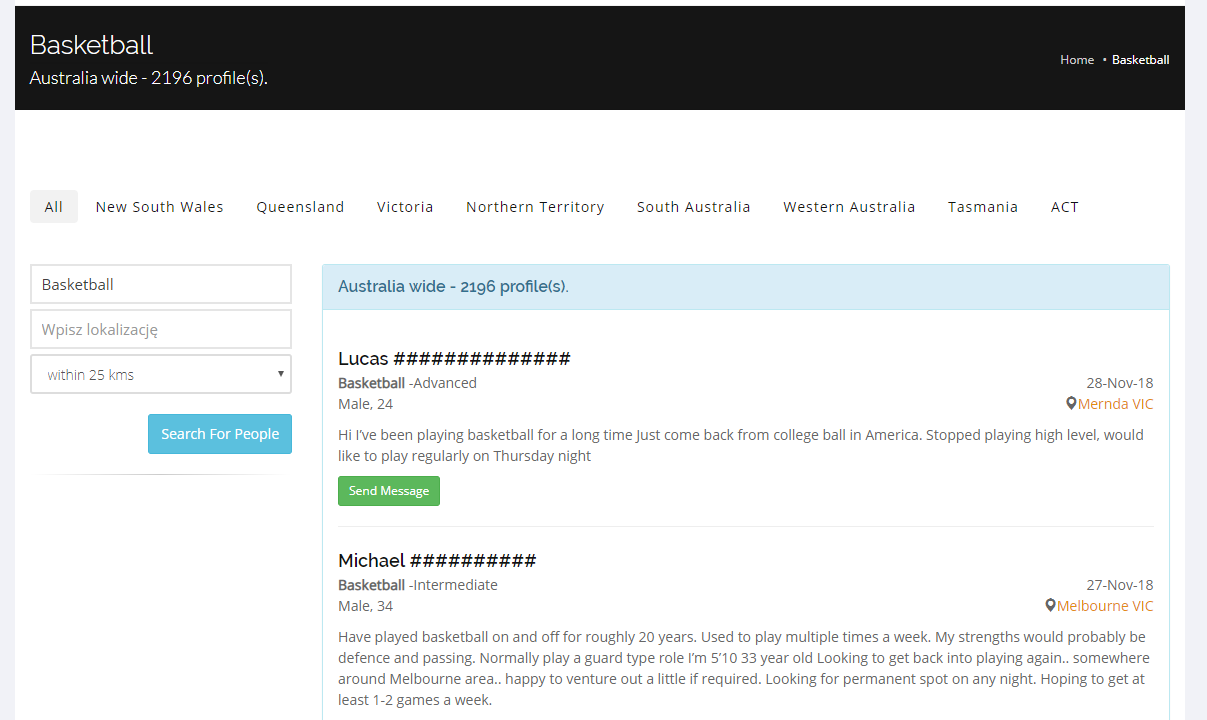
\includegraphics[width=\linewidth]{02-istniejace-rozwiazania/rys/ss-austr.PNG}
\caption{Przykładowe wyniki wyszukiwania osób grających w koszykówkę}
\label{fig:ss-austr}
\end{figure}
\chapter{Koncepcja systemu Team~Challenge}

\begin{comment}
Projekt koncepcyjny? Koncepcja systemu? Systemu NAZWA_WLASNA
\end{comment}

W niniejszym rozdziale została przybliżona koncepcja głównych funkcjonalności platformy \textit{Team Challenge}. Podczas pracy koncepcyjnej autor pracy miał na względzie główny cel systemu jakim jest zrzeszanie zawodników. Proponowane funkcjonalności mają umożliwić osiągnięcie tego celu. Tworząc koncept autor kierował się znajomością potrzeb grupy docelowej, której sam jest częścią, a niejednokrotnie swoje pomysły weryfikował z innymi zawodnikami.

  
\section{Baza wiedzy}

W celu umożliwienia zrzeszania zawodników sportów zespołowych konieczne jest przechowywanie w systemie bazy wiedzy na temat zawodników, drużyn oraz obiektów sportowych. W~poniższych sekcjach zostaną przybliżone główne założenia dotyczące zbierania poszczególnych danych.
  
\subsection{Baza zawodników}

Zawodnicy uprawiający amatorsko pewną dyscyplinę sportu są podstawową grupą docelową projektowanego systemu oraz elementem budującym społeczność. Podstawową funkcjonalnością systemu będzie rejestracja zawodników. Podczas procesu rejestracji od użytkownika zostaną pobrane dane niezbędne do funkcjonowania systemu.

\subsection{Baza drużyn}

Zawodnicy po utworzeniu profilu będą mogli założyć drużynę lub dołączyć do już istniejącej drużyny poprzez otrzymanie oraz akceptację zaproszenia. Zawodnik zakładający drużynę otrzymuje specjalną rolę - kapitana. Kapitanem drużyny powinna być osoba reprezentatywna oraz posiadająca dobry kontakt z pozostałymi członkami zespołu, ponieważ to kapitan będzie zajmował się poszukiwaniem przeciwników oraz umawianiem spotkań. Warto zaznaczyć, że kapitan drużyny dalej pozostaje zawodnikiem i może brać czynny udział w rozgrywkach. 

\subsubsection{Punkt macierzysty}

Drużyna powinna wybrać lokalizację, która na potrzeby tej pracy oraz systemu nazwana została "punktem macierzystym". Punkt ten w obrębie systemu będzie służył jako punkt referencyjny dla porównywania odległości pomiędzy drużynami, jak również do oceny odległości od obiektów sportowych. Punktem macierzystym może być na przykład ulubione boisko zawodników lub częste miejsce spotkań pobliskie zawodnikom. W przypadku trudności wyboru domyślną lokalizacją jest centrum regionu, w którym została utworzona drużyna.

\subsubsection{Aktywność drużyny}

Dostęp do kluczowych funkcjonalności takich jak szukanie przeciwników oraz rzucanie wyzwań wymaga posiadania przez drużynę minimalnej liczby zawodników zdefiniowanej dla konkretnej dyscypliny sportu. Drużyna spełniająca powyższy wymóg określana jest mianem drużyny aktywnej.

\subsection{Baza obiektów sportowych}

Mając na uwadze docelową grupę docelową projektowanego systemu, jaką są zawodnicy grający amatorsko, system powinien dostarczać bazę obiektów ogólnodostępnych, a przede wszystkim nie wymagających wkładu finansowego. Głównym założeniem w tym zakresie jest umożliwienie zawodnikom zgłaszania obiektów. 

\section{Wspomaganie poszukiwania rywali}

Kluczową funkcjonalnością systemu będzie wspomaganie poszukiwania rywali do gry. Projektując tę funkcjonalność autor pracy miał na względzie, że najważniejszym ogniwem w systemie jest korzystający z niego człowiek. Z tego względu system nigdy będzie podejmował decyzji o~wyborze przeciwnika samodzielnie. Celem systemu będzie wspieranie tego procesu poprzez dostarczanie kapitanowi propozycji przeciwników na podstawie zdefiniowanych przez niego preferencji.


\subsection{Kryteria dopasowania}

Podstawowym kryterium dopasowywania drużyn będzie maksymalizacja satysfakcji z gry. Poziom satysfakcji stanowi jednak kryterium, które jest wręcz niemożliwe do ustalenia wprost. Z tego powodu zostały zdefiniowane przesłanki, które mogą wpływać na większą satysfakcję drużyn z rozgrywki:

\begin{itemize}
\item{przybliżony wiek zawodników,}
\item{przybliżony poziom umiejętności oraz forma zawodników,}
\item{mała odległość między punktami macierzystymi drużyn,}
\item{zachowanie fair-play drużyny przeciwnej,}
\item{dobre wspomnienia po poprzednich rozgrywkach.}
\end{itemize}

Istotne z punktu widzenia kapitana szukającego przeciwników mogą być również czynniki wpływające na możliwość umówienia spotkania. Mogą być to na przykład informacje dotyczące aktywności drużyny przeciwnej, czy na przykład jej preferowane godziny gry.

Przytoczone kryteria powinny zostać uwzględnione w projektowanym mechanizmie wspomaganego wyszukiwania przeciwników. Mechanizm powinien zostać zaimplementowany w~sposób rozszerzalny, aby możliwe było definiowanie nowych kryteriów wraz z potrzebami rozwojowymi systemu.

\subsection{Problem optymalizacji wielokryterialnej}

Problem optymalizacji wielokryterialnej jest rozszerzeniem problemu optymalizacji jednokryterialnej, gdzie poszukiwana jest decyzja optymalna, ze zbioru możliwych decyzji na podstawie jednego kryterium. Problem ten sprowadza się do poszukiwania maksimum (bądź minimum) funkcji oceny danego kryterium \cite{optwielok}. Jeżeli kryterium jest ilościowe, np. maksymalna prędkość samochodu, to podejmując decyzje o zakupie jedynie ze względu na to kryterium naturalnie wybierzemy samochód, który osiąga największą prędkość. 

Często jednak podjecie decyzji może być uwarunkowane większą liczbą czynników, na przykład, w przypadku samochodu może to być jego cena, koszt utrzymania, czy czynniki nie ilościowe takie jak jego kolor (w zależności od preferencji kupca). Podejmując decyzje należy rozpatrzyć wiele kryteriów oraz relacje miedzy nimi. Decyzja, która jest optymalna ze względu na jedno z kryteriów, nie musi być optymalna ze względu na pozostałe - z reguły tak nie jest.

\begin{figure}[ht]
\centering
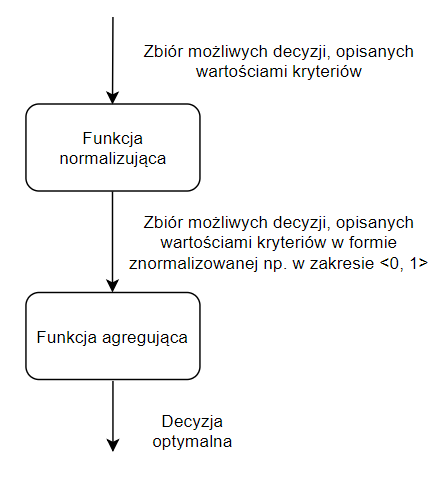
\includegraphics[width=0.5\linewidth]{03-koncept/rys/tradycyjne-algorytmy-opt.PNG}
\caption{Ogólny schemat metody rozwiązywania problemu optymalizacji wielokryterialnej}
\label{fig:diagram-trad-alg-opt}
\end{figure}

Tradycyjnym sposobem rozwiązania problemu jest w pierwszej kolejności znormalizowanie wartości kryteriów do przedziału wartości <0,1>, a następnie dokonanie wyboru korzystając z~wybranej funkcji agregującej \cite{optwielok}. Ogólny schemat został przedstawiony na rysunku ~\ref{fig:diagram-trad-alg-opt}.

Problem podobnej natury występuje w projektowanym systemie. Poszukiwanie rywali do gry można sprowadzić do poszukiwania najlepszych decyzji wyboru drużyny spośród kwalifikujących się drużyn zdefiniowanych w systemie. Przykładowe kryteria wpływające na wartość funkcji oceny dla poszczególnych decyzji (rywali) zostały zdefiniowane w poprzedniej sekcji.

\begin{comment}
\subsection{Rozszerzenie tradycyjnego algorytmu}

Proponując algorytm należy mieć na uwadze domenę problemu oraz charakter danych, na jakich będzie on operował. W związku z tym do tradycyjnego schematu oceny rozwiązań zostanie wprowadzona modyfikacja.

 Normalizacja poszczególnych kryteriów będzie przebiegać przy użyciu różnych funkcji, dopasowanych do charakteru danych. Przykładem uzasadniającym konieczność zastosowania takiej modyfikacji może być porównanie dwóch kryteriów: odległości drużyn oraz średniego wieku zawodników. O ile kryterium odległości może być normalizowane w pełni liniowo, o tyle dla różnicy wieku taka metoda normalizacji jest błędna. Różnica wieku między dwoma zawodnikami, którzy mają 15 oraz 20 lat jest znacznie bardziej istotna aniżeli różnica między zawodnikami w wieku 30 oraz 35 lat - nie można tutaj zastosować operatora liniowego. Dodatkowo w domenie problemu można wyróżnić kryteria nieliczbowe - cechy drużyny, które mogą mieć duży wpływ na jakość dopasowania, np. zadeklarowana chęć ponownej gry z daną drużyną.   

\subsection{Metoda ważonych kryteriów}

Metoda ważonych kryteriów polega na opisaniu funkcji oceny decyzji jako sumy ważonej ocen poszczególnych kryteriów [?]. Konieczne jest przyporządkowanie wagi dla każdego z kryteriów. Ocena poszczególnych decyzji obliczana jest według wzoru: 

\begin{equation}\label{eq:mwk}
F(x)=\sum_{i=1}^{k}w_{i}f_{i}(x)
\end{equation}

gdzie k - ilość kryteriów, x - wektor rozwiązań, $w_{i}$ - wagi takie że:

\begin{equation*}
w \in [0, 1] \mbox{ oraz } \sum_{i=1}^{k}w_{i} = 1
\end{equation*}

Metoda ta została wybrana ze względu na możliwość dynamicznego doboru wag poszczególnych kryteriów. Niektóre z tych wag będą dobierane przez kapitana zgodnie z preferencjami jego drużyny. Rysunek~\ref{fig:diagram-alg-ext} przedstawia schemat działania algorytmu przewidzianego w systemie.


\begin{figure}[H]
\centering
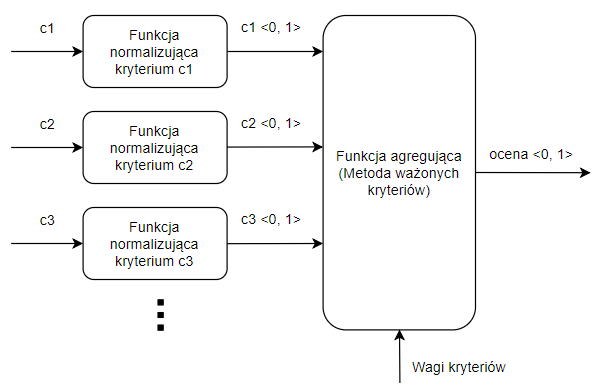
\includegraphics[width=0.8\linewidth]{03-koncept/rys/algorytm.PNG}
\caption{Rozszerzony schemat algorytmu oceny decyzji}
\label{fig:diagram-alg-ext}
\end{figure}
\end{comment}

\section{Wspomaganie umawiania się na rozgrywkę}

Kolejną bazową funkcjonalnością systemu będzie wspieranie przebiegu umawiania spotkań. Kapitan aktywnej drużyny będzie miał możliwość rzucenia wyzwania innej aktywnej drużynie. Kapitan wyzwanej drużyny będzie mógł podjąć decyzję o odrzuceniu wyzwania. W przeciwnym wypadku rozpocznie się proces negocjacji terminu oraz miejsca spotkania. 

\subsection{Negocjacja terminu oraz miejsca spotkania}

Kapitanowie drużyn, komunikując się ze swoimi zawodnikami, będą mogli dodawać do puli ofert swoje propozycje składające się z daty, godziny oraz miejsca spotkania. Miejscem spotkania może być dowolny obiekt sportowy zgłoszony w tym samym regionie co drużyny.  Negocjacje spotkania będą uznane za zakończone w momencie gdy jeden z kapitanów zaakceptuje propozycję drużyny przeciwnej. Termin oraz miejsce zawarte w zaakceptowanej ofercie staną się planowanym terminem oraz miejscem spotkania, a wyzwanie otrzyma status zaakceptowanego.

\begin{figure}[ht]
\centering
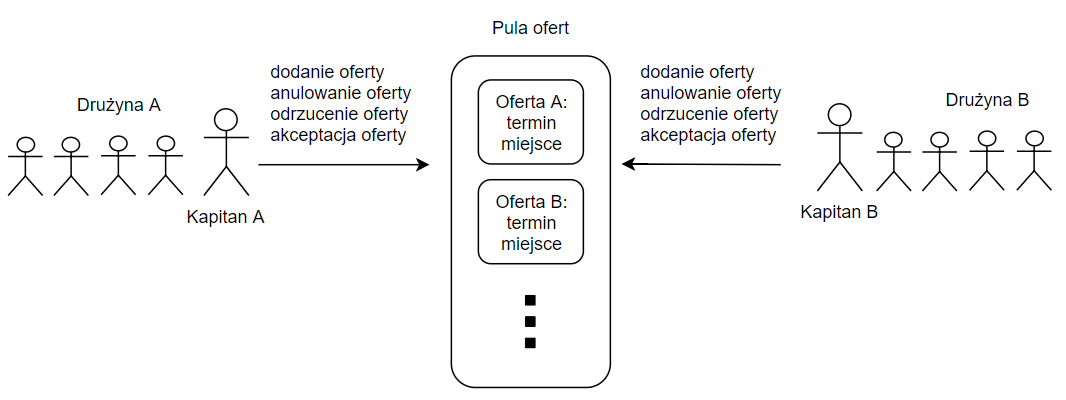
\includegraphics[width=\linewidth]{03-koncept/rys/offer-pool.PNG}
\caption{Koncepcyjny diagram negocjacji przy użyciu puli ofert}
\label{fig:diagram-alg-ext}
\end{figure}

\subsection{Wyniki spotkań}

Wyzwanie zostanie uznanie za zakończone gdy nastąpi wprowadzenie do systemu jego wyniku. Wynik będzie wprowadzony przez dowolną z drużyn biorących udział w wyzwaniu. Wprowadzony wynik powinien zostać poddany weryfikacji przez drugiego z kapitanów, który może go potwierdzić, bądź w przypadku niezgodności, odrzucić. Wynikiem jest ilość punktów zdobytych przez poszczególne drużyny. W przypadku gdy są to dwie różne liczby wyzwanie zakończy się zwycięstwem drużyny, która zdobyła ich więcej. W przeciwnym razie wynikiem wyzwania będzie remis.

\subsection{Ocena drużyn}

Kapitanowie drużyn będą mieli możliwość oceny drużyny rywali po zakończonym spotkaniu. Wypełnienie formularza ma na celu dostarczenie do systemu danych, które mogą poprawić jakość wyszukiwania drużyn. Przykładowymi pytaniami mogą być tutaj: ocena poziomu fair-play drużyny oraz deklaracja chęci ponownej rozgrywki w przyszłości. Ze względu na umożliwienie swobodnej oraz szczerej odpowiedzi oceny nie mogą być widoczne dla ocenianych drużyn.

\chapter{Projekt systemu}

W niniejszym rozdziale ...

> Grupa docelowa, Wymagania funkcjonalne, Przypadki użycia, UML, ERD itp


\chapter{Architektura i technologie}

Niniejszy rozdział został poświęcony ogólnemu opisowi architektury systemu oraz zastosowanych technologii. Dla poszczególnych wyborów zostały przedstawione przesłanki, którymi kierował się autor tej pracy. 

Istotnym czynnikiem mającym wpływ na wybór technologii oraz wzorców architektonicznych była chęć poszerzenia wiedzy autora niniejszej pracy w ich zakresie. Cechą wspólną wszystkich zastosowanych rozwiązań jest szeroki dostęp do materiałów w postaci dokumentacji oraz pozycji książkowych. 

\section{Architektura systemu}

Ze względu na potrzebę szerokiej dostępności platformy została ona zrealizowana jako system webowy w architekturze klient - serwer. Interfejsem użytkownika końcowego jest aplikacja kliencka typu SPA - Single Page Application uruchamiana w przeglądarce internetowej. Aplikacja ta komunikuje się z API wystawionym przez aplikację backendową umieszczoną na serwerze w sieci.  Aplikacja backendowa z kolei komunikuje się z bazą danych w celu odczytu oraz zapisu informacji. 

\begin{figure}[ht]
\centering
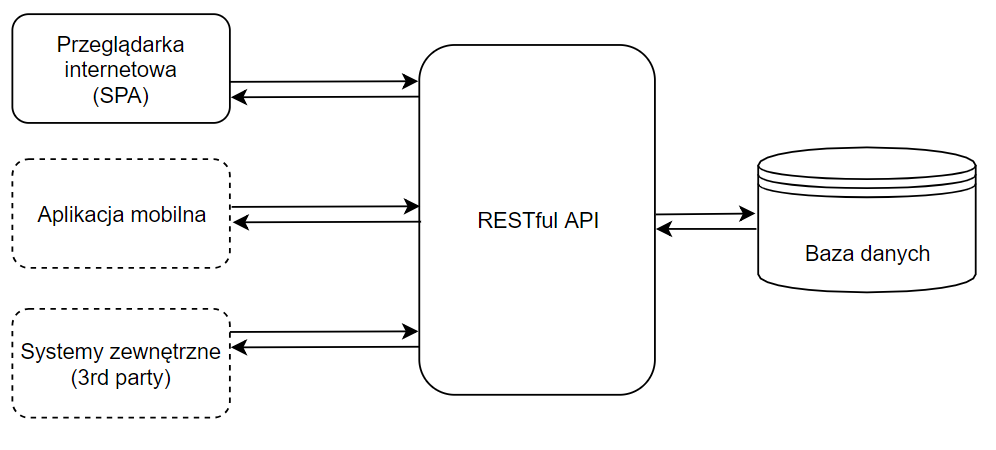
\includegraphics[width=0.8\linewidth]{05-architektura-i-technologie/rys/ogolna-architektura.PNG}
\caption{Diagram ogólnej architektury systemu}
\label{fig:diagram-og-architekt}
\end{figure}

Elementy otoczone linią kreskowaną na diagramie nie są przedmiotem tej pracy, jednak podkreślają uniwersalność API oraz wskazują możliwości rozwojowe oraz integracyjne systemu.

\subsection{RESTful API}
API wystawiane przez część serwerową zostało zaprojektowane w oparciu styl architektoniczny REST, który zakłada komunikację klient-serwer z uwzględnieniem następujących zasad: 
\begin{itemize}
\item użycie podstawowych metody protokołu HTTP czyli - GET, PUT, POST oraz DELETE,
\item identyfikacja zasobów poprzez URL,
\item komunikacja bezstanowa (brak sesji).
\end{itemize}

Użycie podstawowych metod protokołu HTTP pozytywnie wpływa na czytelność oraz intuicyjność API. Projektowanie z uwzględnieniem powyższych zasad pozwala również zminimalizować powiązania pomiędzy serwerem oraz klientem, API staje się uniwersalne. Otwiera to możliwości rozwoju systemu na inne platformy, np. utworzenie aplikacji klienckich dla systemów mobilnych Android oraz iOs. Możliwości rozwoju systemu zostały przedstawione za pomocą zakreskowanych bloków na rysunku~\ref{fig:diagram-og-architekt}

\section{Stos technologiczny}

\subsection{Spring Boot}

Aplikacja backendowa została zaimplementowana w języku Java (w wersji 1.8) z użyciem frameworka Spring Boot (w wersji 2.0.3). Technologie te zostały wybrane ze względu na następujące czynniki:
 \begin{itemize}
\item rozwiązania open source,
\item duże grono użytkowników oraz baza materiałów w sieci,
\item dobra dokumentacja,
\item duża ilość dostępnych modułów Springa np. do komunikacji z bazami danych,
\item chęć poszerzenia wiedzy na temat tych technologii.
\end{itemize}

\subsection{Swagger}

Swagger został wykorzystany do dostarczenia dokumentacji RESTowego API bla bla.

\subsection{JWT}

Technologia Json Web Token została wybrana jako sposób realizacji autoryzacji zapytań do API systemu. JWT jest technologią autoryzacji bezstanowej, przez co bardzo często jest używane do zabezpieczania końcówek REST'owych.

\subsection{MySQL} 

Relacyjna baza danych została wybrana ze względu na przewidywaną dużą ilość powiązań między encjami w systemie. MySQL od firmy Oracle jest darmowym, bezpiecznym oraz wydajnym systemem zarządzania bazą danych.  Istotnym uzasadnieniem wyboru tej technologii jest również bardzo dobra integracja z frameworkiem Spring.

\subsection{Angular}

Główną technologią wykorzystywaną po stronie front endu będzie framework do tworzenia SPA rozwijany przez Google - Angular (w wersji 6.1.0). Framework ten ułatwia budowę skalowalnych i szybkich aplikacji z bogatym interfejsem użytkownika. 

W celu usprawnienia procesu rozwoju aplikacji zostanie wykorzystana biblioteka ngrx (w wersji 6.1.0), wspomagająca zarządzanie stanem aplikacji. Wykorzystanie tej biblioteki znacznie ułatwia analizę działania aplikacji oraz diagnozowanie błędów.

\subsection{AntDesign - NgZorro}

\subsection{Heroku}

\chapter{Implementacja i działanie systemu}



\chapter{Ocena użyteczności}

\begin{comment}
OCENA PRZYDATNOSCI UZYTECZNOSCI WALIDACJA
\end{comment}

System został dwukrotnie poddany walidacji. Pierwszy etap testów odbył się po ukończeniu implementacji pierwszego prototypu systemu. Drugi etap odbył się po ukończeniu drugiego prototypu, który poprawiał niedoskonałości odkryte podczas pierwszego etapu. 
Głównym celem przeprowadzonego procesu walidacji było sprawdzenie, czy implementowane rozwiązanie spełnia oczekiwania potencjalnych odbiorców. 

Do walidacji wytypowane zostały dwie funkcjonalności istotne dla działania systemu. Pierwszą z nich jest proces, który musi przejść każdy nowy użytkownik systemu, czyli tworzenie profilu zawodnika. Drugą z wybranych funkcjonalności jest poszukiwanie rywali oraz rzucanie im wyzwania. Jest to najważniejsza funkcja systemu zawierająca elementy interfejsu wymagające sprawdzenia użyteczności.


\section{Metodyka testów}

Testy odbyły się w formie badań moderowanych, czyli z udziałem osoby nadzorującej ich przebieg \cite{usstudywhatis}. Moderatorem w przypadku wszystkich badań był autor tej pracy. Rolą moderatora w przypadku takich badań jest obserwacja akcji podejmowanych przez osobę wykonującą zadania w systemie oraz sporządzanie notatek.

Do badań zostały wybrane osoby potencjalnie zainteresowane tematem, czyli osoby uprawiające sporty zespołowe. W celu zbadania użyteczności systemu dla różnych grup wiekowych zaproszono osoby w przedziale od 17 do 35 lat. Wśród ankietowanych były osoby profesjonalnie zajmujące się systemami webowymi jak również osoby spoza tej branży. Zgodnie z zaleceniami odnalezionymi w literaturze, w każdym z etapów badań wzięło udział pięciu respondentów \cite{usabilitystudy}.

Dla uczestników badania została przygotowana ankieta składająca się z trzech części. Pierwsza część była ankietą wstępną uzupełnianą przed badaniami. Zawierała ona krótkie wprowadzenie do systemu oraz pytania dotyczące wieku, profesji oraz umiejętności obsługi komputera osoby ankietowanej. Kolejne dwie części zawierały opisy zadań przygotowanych dla użytkowników oraz pytania kontrolne dotyczące intuicyjności poszczególnych procesów. 

Uczestnicy badania zostali poinformowani o tym, że obiektem badania jest interfejs systemu, a nie oni sami. Ze względu na obecność moderatora osoby uczestniczące w badaniu zostały poproszone o głośne myślenie oraz wyrażanie uwag. Moderator podczas badań na bieżąco notował istotne akcje podejmowane przez użytkowników oraz ich uwagi. Po wykonaniu zadań miała miejsce krótka dyskusja na temat zalet interfejsu, napotkanych problemów w obsłudze oraz potencjalnych usprawnień. Na podstawie notatek moderatora oraz ankiet zostały wyciągnięte wnioski dotyczące dalszego rozwoju interfejsu.

\section{Przebieg i wyniki badań}

W pierwszej kolejności do systemu zostały wprowadzone przykładowe (zmyślone) dane zawodników, drużyn oraz obiekty sportowe. Umożliwiło to wykonanie testów wymagających interakcji z innymi obiektami w systemie.

W poniższych sekcjach został opisany przebieg oraz wyniki badań poszczególnych funkcjonalności systemu. Szczegółowe wyniki w postaci złożonych ankiet oraz sporządzonych notatek można znaleźć na załączonej płycie.

\subsection{Tworzenie profilu zawodnika}

W ramach pierwszego zadania ankietowani zostali zalogowani na przygotowane konta użytkowników w systemie, a następnie poproszeni utworzenie profilu zawodnika. Krokami prowadzącymi do wykonania zadania było odnalezienie odpowiedniego formularza a następnie wypełnienie go. 

\subsubsection{Odnalezienie funkcjonalności}

Użytkownicy nie mieli problemów z odnalezieniem kreatora zawodnika. Dwie osoby zasugerowały, że formularz mógłby pokazywać się od razu po pierwszym logowaniu do systemu. Uwaga ta została uwzględniona w implementacji drugiego prototypu. 

\begin{figure}[H]
\centering
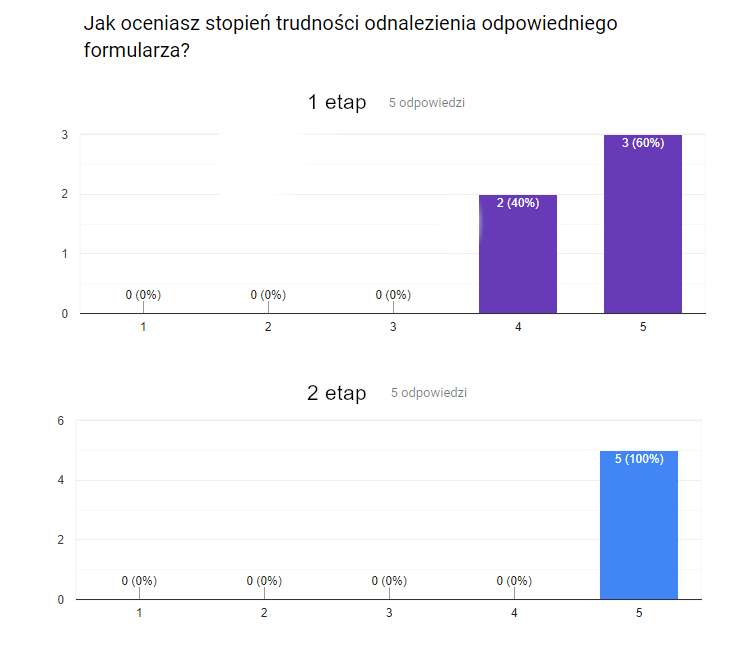
\includegraphics[width=0.8\linewidth]{07-walidacja/rys/survey-create-player.png}
\caption{Zestawienie ocen trudności odnalezienia formularza tworzenia zawodnika po pierwszym etapie badań (1 - bardzo trudne, 5 - bardzo łatwe)}
\label{fig:view-player-skill}
\end{figure}


\subsubsection{Nawigacja po formularzu}

Nawigacja po formularzu składającym się z paru kroków nie sprawiła żadnych problemów respondentom.

\subsubsection{Deklaracja poziomu umiejętności}

Krok polegający na deklaracji poziomu umiejętności również nie stanowił żadnych trudności. Każdy z ankietowanych był w stanie czytając opisy poszczególnych profili umiejętności dopasować się do jednego z nich. Dokonywanie wyborów poprzez przesunięcie suwaków było w pełni intuicyjne.
  
  \begin{comment}
\begin{figure}[H]
\centering
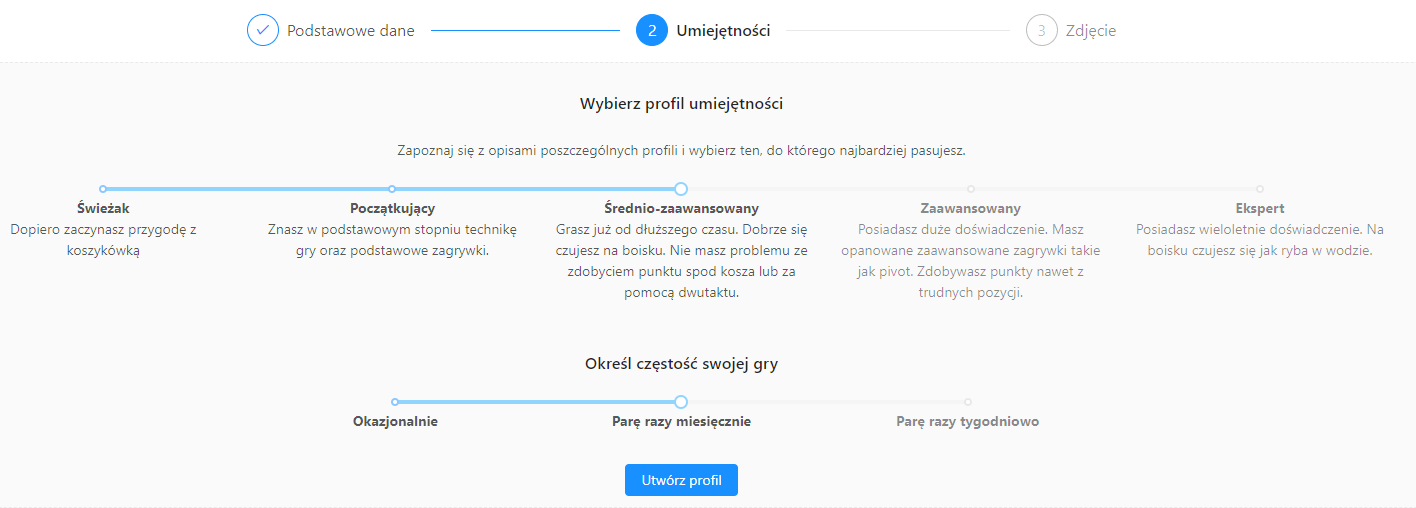
\includegraphics[width=\linewidth]{07-walidacja/rys/p_skill.PNG}
\caption{Widok po zalogowaniu się kapitana do systemu}
\label{fig:view-player-skill}
\end{figure}
\end{comment}

\subsection{Szukanie przeciwników i rzucanie wyzwania}

Drugie zadanie miało na celu sprawdzenie intuicyjności poszukiwania przeciwników oraz tworzenia wyzwania. Respondenci zostali zalogowani na przygotowane wcześniej konto kapitana jednej z drużyn i poproszeni o odnalezienie przeciwników o podobnym wieku w okolicy oraz rzucenie im wyzwania.

\subsubsection{Odnalezienie funkcjonalności}

Respondenci używający pierwszego prototypu odnaleźli odpowiedni formularz, jednak dla niektórych wymagało to trochę czasu. W drugim prototypie odnośnik umieszczono w centrum strony społeczności widocznej po zalogowaniu do systemu.

\begin{figure}[H]
\centering
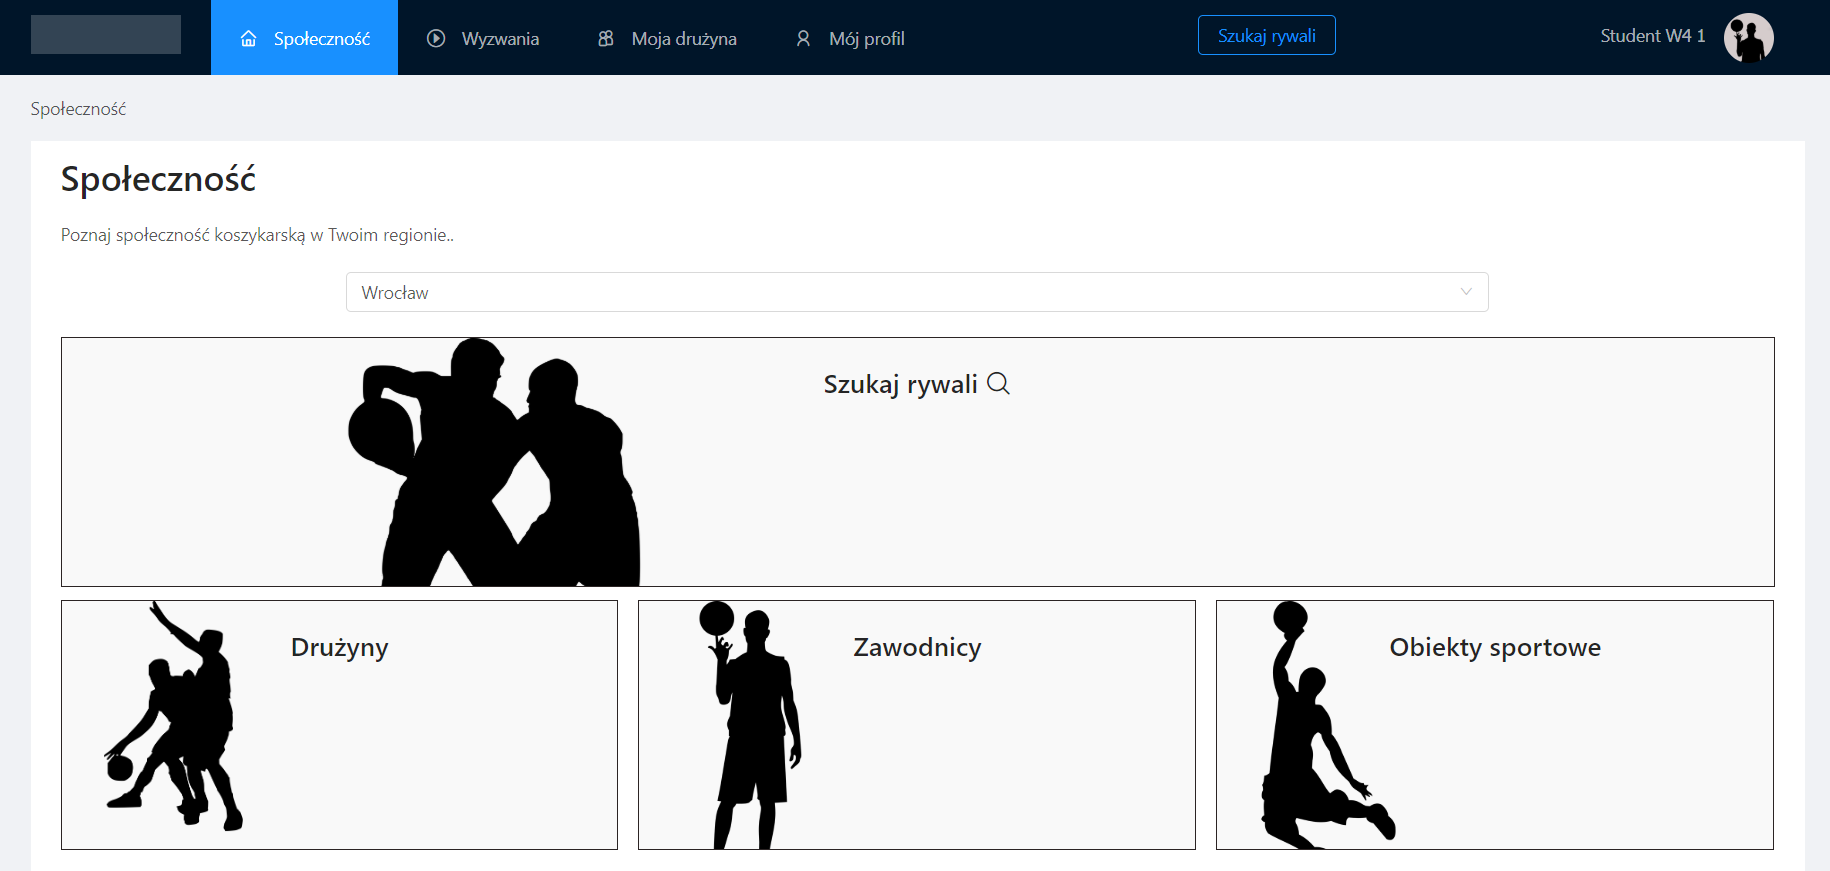
\includegraphics[width=\linewidth]{07-walidacja/rys/spolecznosc.PNG}
\caption{Widok po zalogowaniu się kapitana do systemu}
\label{fig:view-player-skill}
\end{figure}

\subsubsection{Deklaracja preferencji wyszukiwania}

Deklaracja preferencji odnośnie rywali okazała się być problematyczna dla części użytkowników. Zaproponowany w ramach pierwszego prototypu podział procentowy wprowadzał użytkowników w błąd. Z punktu widzenia algorytmu im bardziej znaczące jest dane kryterium tym większą wartość (wagę) powinno ono otrzymać. Użytkownicy jednak wartość 0\% utożsamiali z~brakiem różnicy a więc dobrym dopasowaniem. Z tego względu niektórzy respondenci ustawili suwaki odwrotnie niż było to wskazane. Interfejs przedstawiono na rysunku \ref{fig:suwaki-bef}

Dużą część uwagi podczas przygotowywania drugiego prototypu poświęcono poprawie intuicyjności tej funkcjonalności. W pierwszej kolejności przygotowano makietę nowego wyglądu i opisu funkcjonalności, która została przedstawiona respondentom i spotkała się z ich aprobatą. Następnie planowane zmiany zostały zaimplementowane i zweryfikowane podczas testów drugiego prototypu. Głównym usprawnieniem było zrezygnowanie z wartości procentowych na rzecz abstrakcji - punktów preferencji. Dodatkowo dodano symbole graficzne, dokładniejsze opisy poszczególnych wyborów oraz panel z pomocą odnośnie rozdzielania punktów preferencji. Interfejs po zmianach przedstawiono na rysunku \ref{fig:suwaki-aft}. 


\begin{figure}[H]
\centering
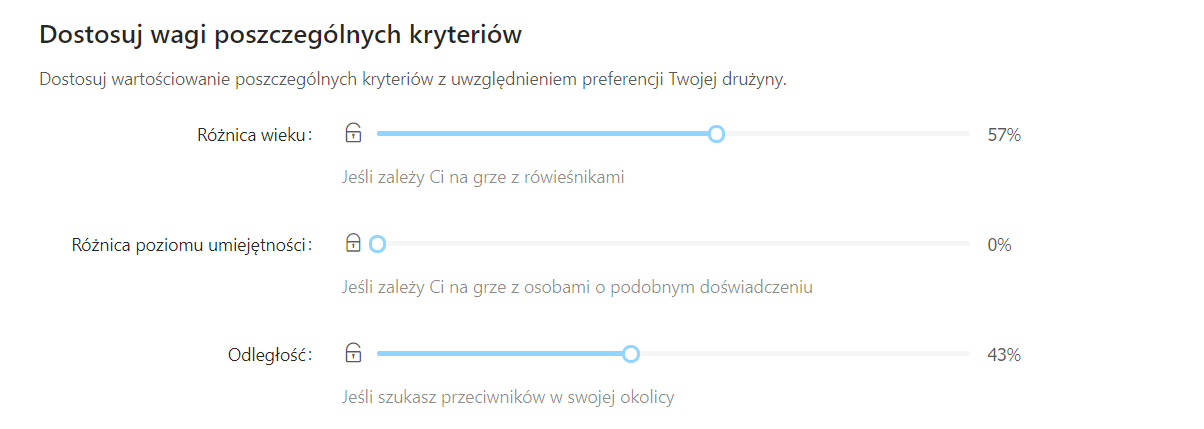
\includegraphics[width=\linewidth]{07-walidacja/rys/suwaki_before_close.PNG}
\caption{Formularz deklaracji preferencji przed zmianami - I prototyp}
\label{fig:suwaki-bef}
\end{figure}


\begin{figure}[H]
\centering
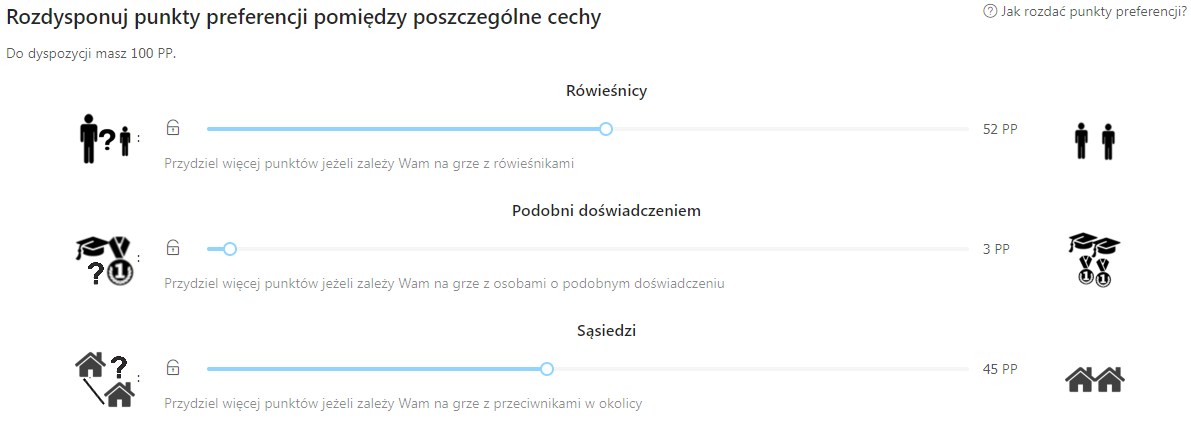
\includegraphics[width=\linewidth]{07-walidacja/rys/suwaki_after_close.PNG}
\caption{Formularz deklaracji preferencji po zmianach - II prototyp}
\label{fig:suwaki-aft}
\end{figure}

Wprowadzone usprawnienia przełożyły się na znaczne lepsze zrozumienie funkcjonalności przez respondentów. Rysunek \ref{fig:survey-suwaki} przedstawia zestawienie odpowiedzi osób ankietowanych przed oraz po wdrożeniu zmian.

\begin{figure}[H]
\centering
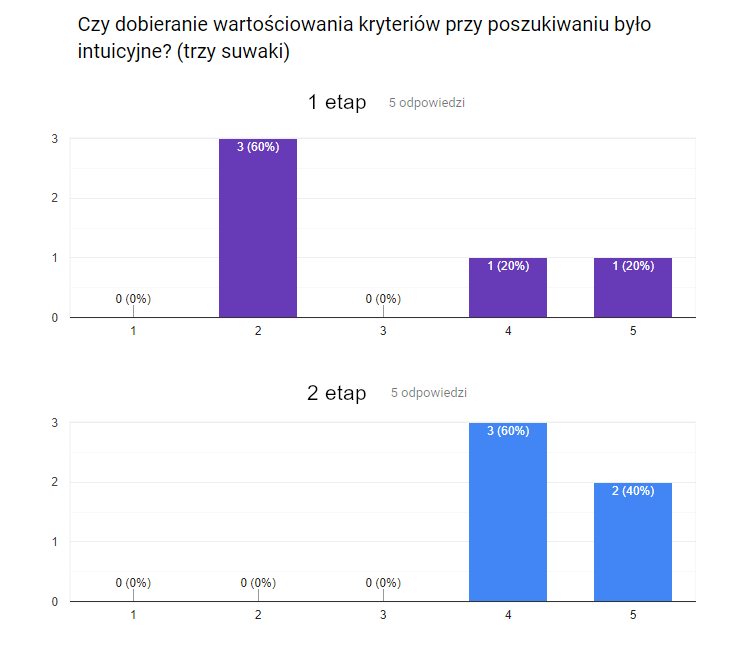
\includegraphics[width=\linewidth]{07-walidacja/rys/survey-search.png}
\caption{Zestawienie ocen intuicyjności deklaracji preferencji wyszukiwania (1 - nie intuicyjne, 5 - w pełni intuicyjne)}
\label{fig:survey-suwaki}
\end{figure}

\begin{comment}
\begin{figure}[H]
\centering
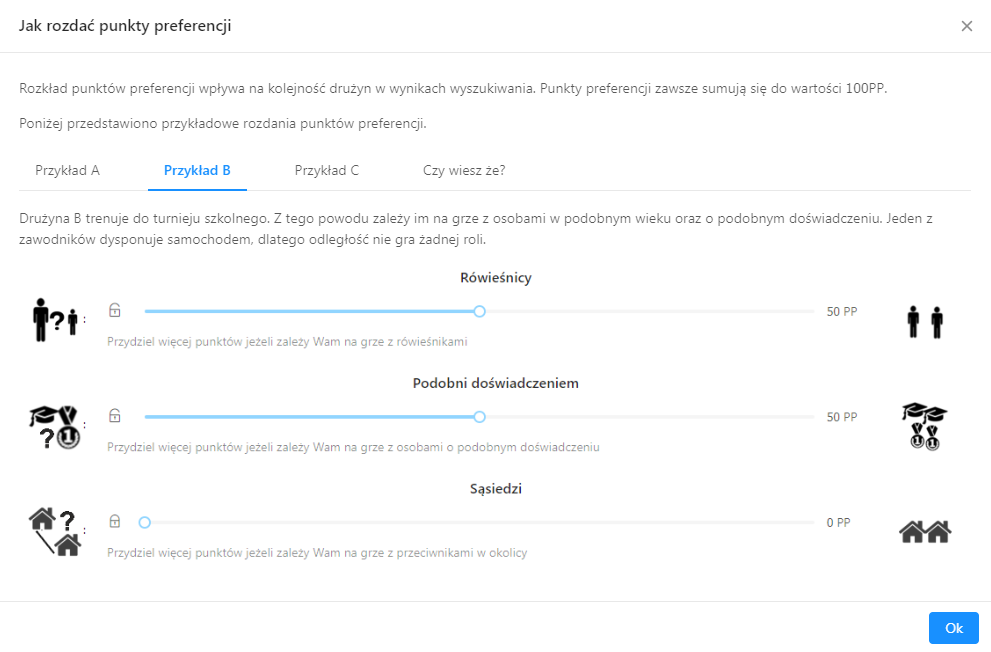
\includegraphics[width=\linewidth]{07-walidacja/rys/help.PNG}
\caption{Aaaaaa}
\label{fig:suwaki-help}
\end{figure}
\end{comment}

\subsubsection{Wyniki wyszukiwania oraz rzucanie wyzwania}

Sposób przedstawienia wyników wyszukiwania - proponowanych rywali okazał się być bardzo przystępny dla użytkowników. Respondenci byli w stanie na podstawie dostarczonych informacji wnioskować na temat dopasowania poszczególnych drużyn, a następnie rzucić wyzwanie jednej z nich. Proponowanie wstępnych ofert miejsca oraz czasu spotkania było zrozumiałe. W ramach tej części funkcjonalności w drugim prototypie zostały wprowadzone jedynie drobne zmiany. 

\chapter{Perspektywy rozwoju}

Podczas trwania prac nad projektem narodziło się wiele pomysłów mogących urozmaicić działanie platformy. W niniejszym rozdziale zostaną przedstawione wybrane kierunki, które mogłyby wpłynąć na atrakcyjność oraz jakość systemu.

\section{Dalszy rozwój interfejsu użytkownika}

O pomyśle na dalsze badania itp.

\section{Aplikacja mobilna}

Naturalnym kierunkiem rozwoju w przypadku platformy internetowej jest dostarczenie użytkownikom aplikacji mobilnej. Rozwiązanie takie ułatwiłoby użytkownikom dostęp do systemu z różnych lokalizacji. Aplikacja również mogłaby za pomocą powiadomień informować użytkowników o nowych zdarzeniach dotyczących umawianych wyzwań.

\section{Partnerskie obiekty sportowe}

Kolejną perspektywą jest nawiązanie współpracy z partnerami w postaci zarządców obiektów sportowych z ograniczonym dostępem. Ideą współpracy byłaby reklama obiektu sportowego w zamian za udostępnienie obiektu w określonych godzinach dla drużyn Team Challenge. Do systemu mógłby zostać wprowadzony nowy typ obiektów sportowych - obiekty partnerskie, wymagające uprzedniej rezerwacji. Należałoby również ograniczać dostęp do takich obiektów, na przykład poprzez wprowadzenie wirtualnej wewnątrz-systemowej waluty w postaci tokenów, którymi drużyny płaciłyby za rezerwację obiektów. Drużyny mogłyby otrzymywać tokeny co jakiś czas oraz za zakończone wyzwania.

\section{System rankingowy}

Interesującym kierunkiem rozwoju jest zdefiniowanie systemu rankingowego drużyn. Wyniki rozgrywek pomiędzy drużynami mogłyby wpływać na pozycję rankingową drużyny. Pozycja rankingowa drużyny mogłaby stanowić nowe kryterium dla algorytmu podczas poszukiwania rywali. Przykładowym systemem rankingowym, który mógłby znaleźć tutaj zastosowanie jest system ELO, używany w rozgrywkach szachowych oraz wielu grach komputerowych online.

\begin{comment}

proponowanei spotkan przez zawodnikow
propozycje pobliskich obiektow przy negocjacjach miejsca
system notyfikacji

\end{comment}
\chapter{Podsumowanie}



%\bibliographystyle{plalpha}
\bibliographystyle{plabbrv}


%UWAGA: bibliotekę referencji należy przygotować samemu. Dobrym do tego narzędziem jest JabRef.
%       Nazwę przygotowanej biblioteki wpisuje się poniżej bez rozszerzenia 
%       (w tym przypadku jest to "dokumentacja.bib")
\bibliography{bibliografia}
\appendix
\chapter{Tytuł dodatku}
Zasady przyznawania stopnia naukowego doktora i doktora habilitowanego w Polsce określa ustawa z dnia 14 marca 2003 r. o stopniach naukowych i~tytule naukowym oraz o stopniach i~tytule w zakresie sztuki (Dz.U. nr 65 z 2003 r., poz. 595 (Dz. U. z 2003 r. Nr 65, poz. 595). Poprzednie polskie uregulowania nie wymagały bezwzględnie posiadania przez kandydata tytułu zawodowego magistra lub równorzędnego (choć zasada ta zazwyczaj była przestrzegana) i zdarzały się nadzwyczajne przypadki nadawania stopnia naukowego doktora osobom bez studiów wyższych, np. słynnemu matematykowi lwowskiemu – późniejszemu profesorowi Stefanowi Banachowi. 

W innych krajach również zazwyczaj do przyznania stopnia naukowego doktora potrzebny jest dyplom ukończenia uczelni wyższej, ale nie wszędzie.


\chapter{Opis załączonej płyty CD}

W poniższych podpunktach opisano zawartość poszczególnych katalogów, które można odnaleźć na załączonej płycie CD.\\

\begin{itemize}

\item \textbf{1-dokument} - Katalog zawierający niniejszą pracę dyplomową w formacie PDF (ang. \textit{Portable Document Format}).  \\

\item \textbf{2-kod-aplikacji-serwerowej} - Katalog zawierający kompletny kod aplikacji serwerowej wraz z metadanymi systemu kontroli wersji \textit{GIT}.   \\


\item \textbf{3-skrypty-baza} - Katalog zawierający skrypty SQL służące do wdrożenia schematu bazy oraz wgrania przykładowych danych.   \\

\item \textbf{4-kod-aplikacji-klienckiej} - Katalog zawierający kompletny kod aplikacji klienckiej wraz z metadanymi systemu kontroli wersji \textit{GIT}.   \\

\item \textbf{5-zrzuty-ekranu} - Katalog zawierający zrzuty ekranu prezentujące działanie zaimplementowanego systemu.   \\

\item \textbf{6-ankiety} - Katalog zawierający ankiety wypełnione przez uczestników badań moderowanych oraz notatki moderatora.   \\

% \item \textbf{7-dokumentacja-api} - Katalog zawierający dokumentację REST API wygenerowaną za pomocą technologii \textit{Swagger}.   \\

\item \textbf{7-dostepy} - Katalog zawierający plik tekstowy z dostępami w postaci adresu wdrożonego systemu oraz danych dostępowych użytkowników testowych.

\end{itemize}





\chapterstyle{noNumbered}
\phantomsection % sets an anchor
\addcontentsline{toc}{chapter}{Indeks rzeczowy}
\printindex

\end{document}
